%%%%%%%%%%%%%%%%%%%%%%%%%%%%%%%%%%%%%%%%%%%%%%%%%%%%
\section{Informed Plan Selection}\label{sec:coverage}
%%%%%%%%%%%%%%%%%%%%%%%%%%%%%%%%%%%%%%%%%%%%%%%%%%%%

In this section, we extend our BDI learning so as to include a confidence test
within the plan selection mechanism itself. More concretely, in the new approach,
instead of using the stability measure to ensure that we only record results that
we are confident in, we instead modify our plan selection procedure to take into
account of how confident we are in the current decision tree.
% %
The idea is simple: the confidence on a plan's decision tree increases as the
different possible choices below the plan (in the goal-plan structure) are better
explored.
% %
Note that while the stability mechanism ensures that failure information is
\emph{not recorded} against a decision tree until the corresponding goal-plan
structure is adequately explored; the new approach instead influences how the
decision tree is \emph{use} at plan selection time.


So, with each plan in the goal-plan tree hierarchy, we identify its set of
potential \textit{choices} as the set of all potential execution paths
\textit{below} the plan in the hierarchy. Observe this can easily be computed
offline beforehand.
% %
Roughly speaking, a plan's decision tree is more \textit{informed} for a world
state, if it accounts for a larger number of plan's choices in that state.
% %
Next, we say that a plan has a higher degree of \emph{coverage} when more of its
underlying choices have been explored in the past and accounted in the
corresponding decision tree.
% %
Technically, given a decision tree $T$ for given plan, we define its converge
$c_T(w) \in [0,\ldots,1]$ as the coverage degree of $T$ for world state $w$.
% %
Initially, when the plan has not yet been executed in a world $w$, its coverage
on the state, namely $c_T(w)$, is zero and the agent may not be that confident on
the probability of plan success estimated by the decision tree at $w$. As the
different ways of execution the plan in the world are explored, the value of
$c_T(w)$ approaches $1$. When all choices have been tried, $c_T(w)=1$ and the
agent may rely on the decision tree estimation of success fully.
% %
Put differently, the coverage degree provides a confidence test on the decision
tree.




Next,	 one can define an equation for determining the final plan selection
weight for a plan that is influenced by the above coverage-based confidence measure.
% %
Formally, we define the plan's weight for plan selection, namely $\Omega'(w)$, based
on the plan success expectation returned by the decision tree and the current
coverage degree:
%
\begin{equation*}\label{eqn:coverage}   
\Omega'_T(w) = 0.5 + \left[  c_T(w) *  \left( p_T(w) - 0.5 \right)  \right].
\end{equation*}
	
	
Initially, the weight of the plan for a world where it has never been executed is
assigned a default value ($0.5$ in our case).
% %
As the coverage degree increases with time, by trying the various ways the plan
could be executed, the weight of the plan approaches the true value estimated by
the plan's decision tree.



Regarding how the coverage degree is calculated at every point, we should make
the following two observations.
% %
First, the coverage $c_T(w)$ for a world $w$ is calculated and stored each time a
result is recorded against a plan's decision tree $T$.
% %
Second, it requires, in principle, $\tau \times |S|$ \emph{unique} executions of
a plan for it to reach \emph{full} coverage, where $\chi$ is the total number of
choices below the plan and $|S|$ is the number of possible worlds. Practically,
however, it takes significantly less since choices below a plan are effectively
represented by an AND/OR tree, and each time an AND node fails, the subsequent
nodes are not tried and are accounted covered for the world in question.
% %
Moreover, since plans are typically executed in the context of other plans
(e.g., the plan to check-in is always executed after a plan to go to the
aiport), it would not be necessary to account for the whole world space, but
only for its subset that is relevant for the plan.

\newcommand{\CLSELA}{\mbox{$\CL\!\!+\!\!\Omega$}}
\newcommand{\CLSELB}{\mbox{$\CL\!\!+\!\!\Omega'$}}
\newcommand{\BULSELA}{\mbox{$\BUL\!\!+\!\!\Omega$}}
\newcommand{\BULSELB}{\mbox{$\BUL\!\!+\!\!\Omega'$}}

\medskip With the new account for plans' weight, we (re)considered the two
learning approaches \CL\ and \BUL\ from the previous section with a plan
selection based on such weights. We shall refer to such new agents as \CLSELB\
and \BULSELB, respectively.
% %
Similarly, let us call $\CLSELA$ and $\BULSELA$ the corresponding agents using
the \emph{original} probabilistic selection where the weight of a plan depends
only on its decision tree success expectation $\Omega_T(w) = p_T(w)$.



In Figure~\ref{fig:performance-applicability}, we show the performance of all
four BDI learning agents in structures $\T_2$ and $\T_4$.
% %
First of all, when it comes to the \BUL\ stabibility-based learning scheme, the
two variations, namely $\BULSELA$ and $\BULSELB$, always show similar
performance.
% %
This is not surprising, as the stability test performed by these agents at each
plan node implicitly implies a test of coverage. Indeed, for a plan to become
``stable,'' the agent needs to (substantially) explore all possible  ways of
executing it. Consequently,  until the plan is deemed stable, $\Omega_T$ behaves
like $\Omega_T'$ with coverage $c_T(w)=0$, thus effectively reducing
$\Omega'_T(w)$ to $\Omega_T(w)$.



Second, let us focus on the \CL\ approach.
% %
For the \CL-favouring structure $\T_1$, the performance of \CLSELB matched that
of \CLSELA\ reported in the previous section (cf. Figure~\ref{fig:T1_result}).
% %
This was also the case with the balanced structure $\T_3$ where both \CL\ and
\BUL\ performed equally well under the original plan selection mechanism---the
performance of \CLSELB\ was the same as that reported in
Firgure~\ref{fig:T3_result} for \CLSELA.
% %
Thus, for the cases where \CL\ was performing reasonably well, nothing is lost
when using the new plan selection mechanism.



The situation is completely different, though, when one considers the goal-plan
structure $\T_2$, under which the conservative \BULSELA\ approach used to display
better performance than \CLSELA\ (cf. Figure \ref{fig:T2_result}).
% %
When ran in $\T_2$, the \CLSELB\ approach showed a dramatic improvement over the
\CLSELA-based one. Figure \ref{fig:T2_result2} shows this change with the results
for the new approach to plan selection $\BULSELB$ and $\CLSELB$ superimposed over
the original results from Figure \ref{fig:T2_result} (in grey).
% %
The reason why the new plan selection mechanism improves the \CL\ learning scheme
is that even though the success estimation for plan $P_i$ would still be low
initially (remember that \CL, in contrast with \BUL, would record all initial
failure runs against $P_i$), the agent would not be so confident on such
estimation until the plan's coverage degree increases and it will therefore boost
such estimation towards the default weight of $0.5$. In other words, the false
negative executions collected by the agent for plan $P_i$ would not be
considered so seriously due to low plan coverage. As full coverage is
approached, one would expect the agent to have discovered the success execution
encoded in $P_i$.



\begin{figure*}[t]
\begin{center}
\subfigure[Structure $\T_2$]{\label{fig:T2_result2}
%!TEX root = ../dsingh-aamas10.tex
\begin{tikzpicture}[x=0.00276cm,y=5cm]
    % Draw the axes and grid lines
    \draw[-] (0,0) -- (0,1) -- (3000,1) -- (3000,0) -- cycle; 
    \draw[-,thin, dotted, ystep=0.2, xstep=3000] (0,0) grid (3000,1);
    \foreach \x in {500, 1500, 2500}  \draw [-,xshift=0](\x,4pt) -- (\x,-1pt);
    \foreach \y in {0.0,0.2,0.4,0.6,0.8,1.0}  \draw [-,yshift=0](4pt,\y) -- (-1pt,\y);
    \foreach \x/\xtext in {500/500, 1500/1500, 2500/2500} \node at (\x,0) [below] {$\xtext$};
    \foreach \y/\ytext in {0.0,0.2,0.4,0.6,0.8,1.0}  \node at (0,\y) [left] {$\ytext$};
    \node at (0,1.1) {Success};
    \node at (2700,0.15) {Iterations};
    \draw[-,red] plot[mark=x,mark size=4,mark options={color=red}] 
			file {figs/data/test05v3gm.CC.tikzdata};
    \draw[-,thin,densely dashed,black] plot[mark=x,mark size=4,mark options={color=black}] 
			file {figs/data/test05v3gm.CP.tikzdata};
    \draw[-,thin,densely dashed,black] plot[mark=o,mark size=2,mark options={color=black}] 
			file {figs/data/test05v3gm.SP.tikzdata};
    % Also draw the expected convergence: 0.9^8 actions=0.43046
    \draw[dashed,-,yshift=0](0,0.43046) -- (3000,0.43046);

\end{tikzpicture}

}
\qquad
\subfigure[Structure $\T_4$]{\label{fig:T4_result}
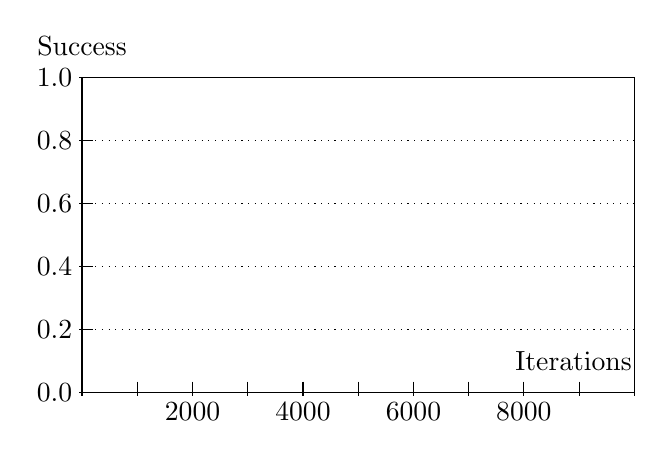
\begin{tikzpicture}[x=0.0007cm,y=4cm]
    % Draw the axes and grid lines
    \draw[-] (0,0) -- (0,1) -- (10000,1) -- (10000,0) -- cycle; 
    \draw[-,thin, dotted, ystep=0.2, xstep=10000] (0,0) grid (10000,1);
    \foreach \x in {0,1000,...,10000}  \draw [-,xshift=0](\x,4pt) -- (\x,-1pt);
    \foreach \y in {0.0,0.2,0.4,0.6,0.8,1.0}  \draw [-,yshift=0](4pt,\y) -- (-1pt,\y);
    \foreach \x/\xtext in {2000/2000, 4000/4000, 6000/6000, 8000/8000} \node at (\x,0) [below] {$\xtext$};
    \foreach \y/\ytext in {0.0,0.2,0.4,0.6,0.8,1.0}  \node at (0,\y) [left] {$\ytext$};
    \node at (0,1.1) {Success};
    \node at (8900,0.1) {Iterations};
    \draw[-] plot[mark=square,mark size=2,mark options={color=black}] 
			file {data/testMultiSolutionsR.CC.tikzdata};
    \draw[-,thin,densely dashed,gray] plot[mark=triangle,gray,mark size=3,mark options={color=gray}] 
			file {data/testMultiSolutionsR.CP.tikzdata};
    \draw[-] plot[mark=diamond,mark size=3,mark options={color=black}] 
			file {data/testMultiSolutionsR.SC.tikzdata};
    \draw[-,thin,densely dashed,gray] plot[mark=o,gray,mark size=2,mark options={color=gray}] 
			file {data/testMultiSolutionsR.SP.tikzdata};

\end{tikzpicture}

}

\caption{Comparison of the new configurations \BUL+$E'$ (diamonds) and \CL+$E'$
(squares) against the earlier \BUL+$E$ (circles) and \CL+$E$ (triangles) for the
\BUL-favouring structure $\T_2$.}
\end{center}
\end{figure*}



Even more interesting is the the impact of the new plan selection mechanism on
agents that work with an applicability threshold, that is, agents that may not
select a plan if they are deemed not worth it. For this cases, the coverage-based
avoids the \CL\ approach judging a plan not worth it based on false negative
experiences. Even if a plan is deemed with very low probability of success, if it
has not been substatially ``covered,'' its weight would still be bias towards the
default value of $.5$. Of course, a consistent agent system should always have
the applicability threashold substantially below the default plan selection
weight.
%%
Figure~\ref{fig:performance-applicability} shows how the new agent systems
using the $\Omega'$ selection weight perform, and in particular, how \CLSELB\
does not suffer from the limitations of its previous \CLSELA\ version.


Finally, we point out that agents based on the new converge-based plan selection
scheme will be able to realize when the optimal solution for a goal has been
reached before the agents based on the original scheme.
% %
This happens because, by using the coverage degree to calculate the final weight
of a plan for a goal, the system is both looking for successful paths while
maximizing    the uniform exploration of the agent's plan library.
% %
So, for example, since $P$ is more ``complex'' than $P_i'$ in in structure $\T_2$
(Figure~\ref{fig:T2}), an agent based on the $\Omega'$ weighting function, will
tend to give more execution chances to the former in order to achieve a more
uniform exploration of the options for goal $G$.


 

Summarizing, the above results are significant in that they suggest that the
alternative plan selection mechanism, which uses the coverage notion as a
confidence test, does provide substantial benefits. In particular, it improves
the \CL\ approach substantially in those cases where it performed poorly due to
false negative experiences, i.e., failure runs for a plan that includes
successful executions.  Being the \CL\  simpler than the \BUL\ one (as no account
of ``stability'' is used), this suggests that the \CLSELB\ combination as the
overall best one.
% %
Nonetheless, it should be noted that there is indeed an instrisic trade-off
between coverage and uniform exploration and decision tree estimation of success
and bias execution towards success. This is, in fact, the standard trade-off
between exploration and explotation when it comes to learning and acting at the
same time.
%%





% \bigskip\bigskip\bigskip
% \textbf{move to discussion??}
% Since the
% coverage $c_T(S)$ in Equation \ref{eqn:coverage} is simply a
% confidence measure, then the way it is \textit{used} will determine
% the weighting of the confidence in the final plan selection
% probability $p'_T(w)$. For instance we could replace $c_T(S)$ in
% Equation \ref{eqn:coverage} with $c_T(S)^{1/b}$ where $b$ is the
% weighting (and $b=1$ gives us the original Equation
% \ref{eqn:coverage}). Then adjusting $b \rightarrow 0, (0 \ne b < 1$)
% we get more \BUL+$E$-like performance, while adjusting $b \rightarrow
% \infty (b > 1)$ will result in more \CL+$E$-like performance. In fact,
% an improved agent could reference the (static) goal-plan tree
% structure at runtime and adjust $b$ automatically based on the offline
% compiled knowledge of which approach works better for which tree
% topology. 
% % This extension is left as a future implementation exercise. 
% 
% We noted earlier in Section \ref{sec:experiments} that plan execution
% in real systems is often not cost-free, so presumably the agent would
% not execute a plan with too low a probability of success. We also show
% that such deliberation does not favour \CL\ but does \BUL. It is clear
% that choosing not to execute a plan below a threshold probability of
% failure would also hurt the \CL+$E'$ configuration (though
% not as much as \CL+$E$). For such systems, we suggest that the
% weighting $b$ be used to get the preferred \BUL-like performance. 


